\documentclass{standalone}
\usepackage{tikz}
\usetikzlibrary{shapes.geometric,fit}
\begin{document}
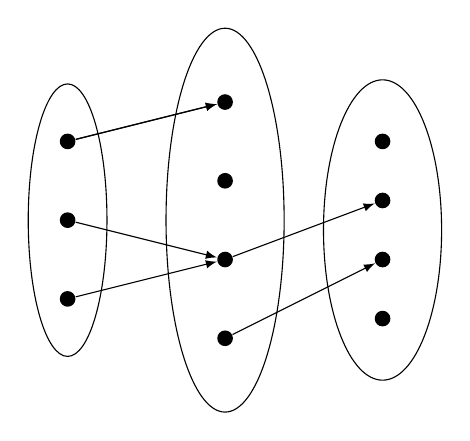
\begin{tikzpicture}
%put some nodes on the left
\foreach \x in {1,2,3}{
\node[fill,circle,inner sep=2pt] (d\x) at (0,\x) {};
}
\node[fit=(d1) (d2) (d3),ellipse,draw,minimum width=1cm] {}; 
%put some nodes on the center
\foreach \x[count=\xi] in {0.5,1.5,...,4}{
\node[fill,circle,inner sep=2pt] (r\xi) at (2,\x) {};
}
\node[fit=(r1) (r2) (r3) (r4),ellipse,draw,minimum width=1.5cm] {}; 
%put some nodes on the right
\foreach \x[count=\xi] in {0.75,1.5,...,3}{
\node[fill,circle,inner sep=2pt] (c\xi) at (4,\x) {};
}
\node[fit=(c1) (c2) (c3) (c4) ,ellipse,draw,minimum width=1.5cm] {};
\draw[-latex] (d1) -- (r2);
\draw[-latex] (d2) -- (r2);
\draw[-latex] (d3) -- (r4);
\draw[-latex] (r1) -- (c2);
\draw[-latex] (r2) -- (c3);
\draw[-latex] (d3) -- (r4);
\end{tikzpicture}
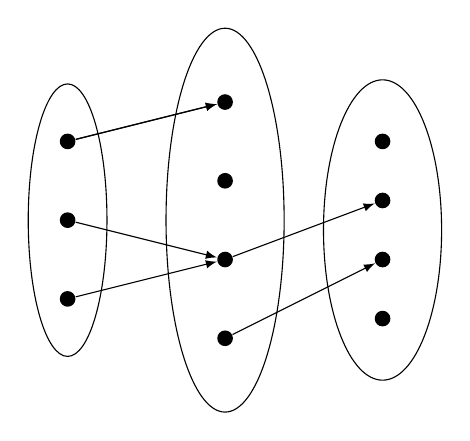
\begin{tikzpicture}
%put some nodes on the left
\foreach \x in {1,2,3}{
\node[fill,circle,inner sep=2pt] (d\x) at (0,\x) {};
}
\node[fit=(d1) (d2) (d3),ellipse,draw,minimum width=1cm] {}; 
%put some nodes on the center
\foreach \x[count=\xi] in {0.5,1.5,...,4}{
\node[fill,circle,inner sep=2pt] (r\xi) at (2,\x) {};
}
\node[fit=(r1) (r2) (r3) (r4),ellipse,draw,minimum width=1.5cm] {}; 
%put some nodes on the right
\foreach \x[count=\xi] in {0.75,1.5,...,3}{
\node[fill,circle,inner sep=2pt] (c\xi) at (4,\x) {};
}
\node[fit=(c1) (c2) (c3) (c4) ,ellipse,draw,minimum width=1.5cm] {};
\draw[-latex] (d1) -- (r2);
\draw[-latex] (d2) -- (r2);
\draw[-latex] (d3) -- (r4);
\draw[-latex] (r1) -- (c2);
\draw[-latex] (r2) -- (c3);
\draw[-latex] (d3) -- (r4);
\end{tikzpicture}
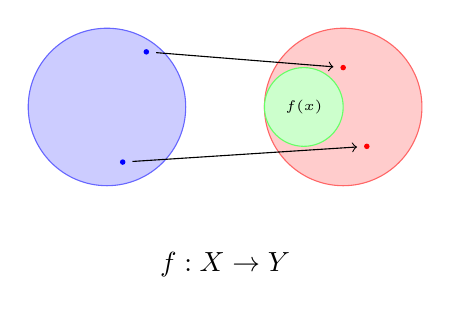
\begin{tikzpicture}
    % draw the sets
    \filldraw[fill=blue!20, draw=blue!60] (-1.5,0) circle (1cm);
    \filldraw[fill=red!20, draw=red!60] (1.5,0) circle (1cm);
    \filldraw[fill=green!20, draw=green!60] (1,0) circle (0.5cm);

    % the texts
    \node at (1,0) {\tiny$f(x)$};
    \node at (0,-2) {$f: X \to Y$};

    % the points in the sets (here I just create nodes to use them later on to position
    % the circles and the arrows
    \node (x1) at (-1,0.7) {};
    \node (x2) at (-1.3,-0.7) {};
    \node (y1) at (1.5,0.5) {};
    \node (y2) at (1.8,-0.5) {};

    % position the elements in the sets (at the nodes we just created)
    \fill[blue] (x1) circle (1pt);
    \fill[blue] (x2) circle (1pt);
    \fill[red] (y1) circle (1pt);
    \fill[red] (y2) circle (1pt);

    % draw the arrows
    \draw[->] (x1) -- (y1);
    \draw[->] (x2) -- (y2);
\end{tikzpicture}
\end{document}